\section{Change in assembly}

\textbf{Created by:} Ali Hasanzadeh \\
\textbf{Modified by:}  \\

\subsection*{Scenario Objective}

This scenario illustrates how to represent the change in an object's association with different assemblies over time using the IOF/BFO ontology framework. It focuses on:
\begin{itemize}
    \item Highlighting the use of temporal regions and temporal intervals to associate an object's presence in specific assemblies over time.
    \item Representing the object's changing relationships to multiple assemblies through different parthood properties.
    \item Using physical connections of components as an outcome some process assembly to denote a material artifacts function(s). 
\end{itemize}

\subsection*{General Pattern Description}

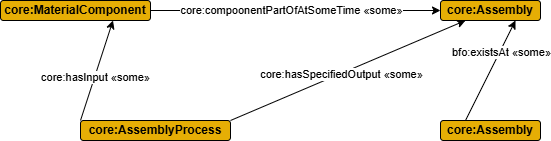
\includegraphics[scale=0.48]{scenarios/assemblies-components/images/assembly-component-general-pattern-description.png}

A material component may be a component of different assemblies at different times. In this scenario, the \cname{core}{MaterialComponent} would be related to multiple \cname{core}{Assembly} via the \opname{core}{componentPartOfAtSomeTime} property. As this connection cannot be true between a \cname{core}{MaterialComponent} and different \cname{core}{Assembly} artifacts at once, we would denote this reality by pairing the \cname{bfo}{TemporalRegion} of each \cname{core}{AssemblyProcess} with the \cname{core}{MaterialComponent}.

\subsection*{Use-Case Pattern Description}
A PLA joint can be part of a modular shelf used for storing books and later be repurposed in another modular shelf used for storing tools. The particular example is chosen to emphasize the difference between assemblies and machines as well. In this scenario, the joint is \opname{core}{componentPartOfAtSomeTime} multiple shelves (\cname{core}{Assembly}). In other words, this \cname{core}{Component} is \opname{core}{componentPartOfAtSomeTime} one \cname{core}{Assembly} shelf at some \cname{bfo}{TemporalRegion} as the result of some \cname{core}{AssemblyProcess} and \opname{core}{componentPartOfAtSomeTime} of another \cname{core}{Assembly} shelf at some other \cname{bfo}{TemporalRegion} as the result of a different \cname{core}{AssemblyProcess}.